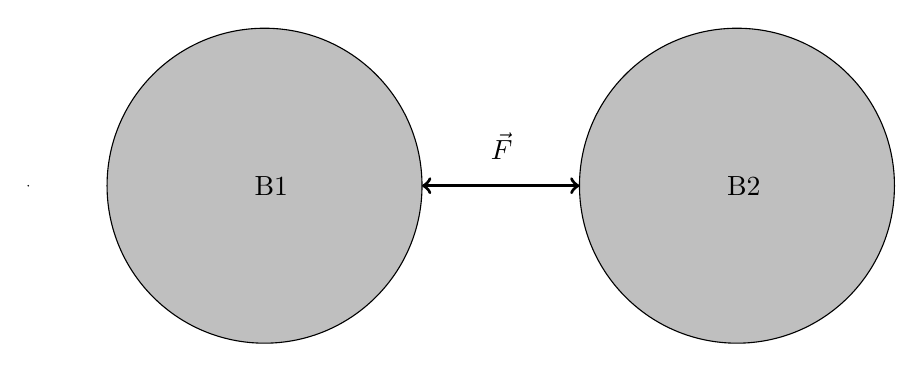
\begin{tikzpicture}
\draw[black] (0,0) circle (0.001cm);
\filldraw[draw = black, fill = lightgray] (3,0) circle (2cm);
\filldraw[draw = black, fill = lightgray] (9,0) circle (2cm);
\draw[very thick, <->] (5,0) -- (7,0);
\draw[black] (5.75,0.5) node[anchor=west] {$\vec{F}$};
\draw[black] (2.75,0) node[anchor=west] {B1};
\draw[black] (8.75,0) node[anchor=west] {B2};
\end{tikzpicture}
\begin{center}
(Figure 3.3.1)
\end{center}

When I was first learning physics, I found the first and second law to be much easier to conceptualize than the 3rd law simply because the first two laws seemed more mathematical. The phasing of the third law in popular parlance is "every action has an equal yet opposite reaction." I frankly believe this is a terrible way to describe the third law. Firstly, it is not at all clear what action and reaction are. Also, we are doing physics here, not chemistry, why are we talking about reactions? The best description I have is that when a body B1 imparts a force  $\vec{F_1}$ on another body(B2). Body B2 must impart a force of magnitude $\vec{F_1}$ but in the opposite direction of $\vec{F_1}$. Please note that this does not refer to a net force, this is only about special forces between objects. One thing the third law tells us is that forces work in both directions. A body can not impart a force on another object without the other body imparting a force on it. This has no parallel in our lives. When we push against something, we do not think of it imparting a force on us but as counter-intuitive as it may seem, this is in fact what is happening. Another interesting example is gravity. The earth acts on us with the force of gravity, and we impart the same force on us. However, because the earth is so massive, our force does not do anything substantive to the earth. $\vec{F} =m\vec{a}$. The force earth imparts on us has magnitude $F$ and causes are the acceleration of $\frac{F}{m}=a=g$. However, The magnitude of the force $F$ is the same for earth but $m_{Earth}$ is much greater than $m_{normal object}$ so $$a_{Earth}=\frac{F}{m_{Earth}}\approx0$$ for all practical considerations.